% Prepared estimation/design mechanism; one shared source for print and web.
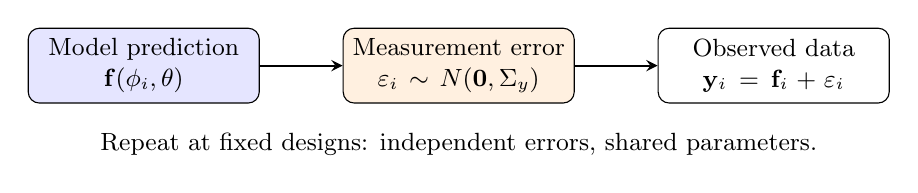
\begin{tikzpicture}[>=stealth, every node/.style={font=\small,align=center}, b/.style={draw,rounded corners,text width=2.7cm,minimum height=.95cm}]
\node[b,fill=blue!10] (f) at (0,0) {Model prediction\\$\mathbf f(\boldsymbol\phi_i,\boldsymbol\theta)$};
\node[b,fill=orange!12] (e) at (4,0) {Measurement error\\$\boldsymbol\varepsilon_i\sim N(\mathbf0,\boldsymbol\Sigma_y)$};
\node[b] (y) at (8,0) {Observed data\\$\mathbf y_i=\mathbf f_i+\boldsymbol\varepsilon_i$};
\draw[->,thick] (f)--(e);\draw[->,thick] (e)--(y);
\node at (4,-1) {Repeat at fixed designs: independent errors, shared parameters.};
\end{tikzpicture}
